\documentclass[sigconf,nonacm]{acmart}

%%% do not modify the following VLDB block %%
%%% VLDB block start %%%
\usepackage{pvldb}
%%% VLDB block end %%%

% Official-template placeholders for an unpublished working draft.
\renewcommand\vldbdoi{XX.XX/XXX.XX}
\renewcommand\vldbpages{XXX-XXX}
\renewcommand\vldbavailabilityurl{}

\usepackage[utf8]{inputenc}
\usepackage{array,multirow}
\usepackage{xurl}
\usepackage{enumitem}
\usepackage{listings}
\usepackage{tikz}
\usetikzlibrary{arrows.meta,positioning}
\newcommand{\SQLReduction}{645.3}
\newcommand{\LatencySpeedup}{59.04}
\newcommand{\BaseLatency}{6,506.320}
\newcommand{\FinalLatency}{110.206}

\hypersetup{pdftitle={Jac DB: From Persistent Graph Walkers to Relational Plans},
 pdfauthor={Working Draft},pdfsubject={Compiler and runtime study with reproduced database measurements},
 pdfkeywords={Jac, graph walkers, database compilation, profiling}}
\newcommand{\jacdb}{Jac DB}
\newcommand{\code}[1]{\texttt{#1}}
\newcommand{\term}[1]{\emph{#1}}
\makeatletter
\newcommand{\tableinput}[1]{\@@input #1 }
\makeatother
\lstdefinelanguage{Jac}{
  morekeywords={walker,node,edge,has,can,with,entry,exit,for,in,if,else,visit,report,here,self,return,def},
  sensitive=true,morecomment=[l]{\#},morestring=[b]",morestring=[b]'
}
\lstset{basicstyle=\ttfamily\scriptsize,keywordstyle=\bfseries,
  commentstyle=\color{black!55},columns=fullflexible,keepspaces=true,
  breaklines=true,breakatwhitespace=false,showstringspaces=false,
  frame=single,rulecolor=\color{black!18},framesep=4pt,
  xleftmargin=4pt,xrightmargin=4pt,aboveskip=7pt,belowskip=5pt}
\title{Jac DB: From Persistent Graph Walkers to Relational Plans}
\author{Working Draft}
\date{October 19, 2026}

\begin{document}

\begin{abstract}
Persistent graph programs express computation as traversals, object reads,
and mutations. A direct implementation can turn a short program into thousands
of database commands. We study a compiler and runtime for Jac that groups
typed traversals, pushes a recognized counting computation into SQL, and delays
object materialization until after ranking. The application retains its graph
program while the execution granularity changes from individual accesses to
batched relational work. On a social-network workload derived from IC5, a
source-controlled reproduction reduces warmed SQL statements from 278,769 to
432 across 20 inputs, a \SQLReduction{}$\times$ reduction. Logging-off median
request latency falls from \BaseLatency{} to \FinalLatency{}\,ms,
a \LatencySpeedup{}$\times$ speedup, with matching checked results. A broader
evaluation covers seven social-network query classes, two transaction types,
and a social application with reads and writes. Detailed write profiling
identifies the remaining cost of repeated anchor loads, traversal queries,
request initialization, and transaction handling. A controlled
\code{ANALYZE}-only intervention also separates a database-statistics effect
from a compiler-version effect, motivating dependency-aware optimization
across traversal continuations.
\end{abstract}

\maketitle

%%% do not modify the following VLDB block %%
%%% VLDB block start %%%
\vldbtopmatter
%%% VLDB block end %%%

\section{Introduction}
\label{sec:introduction}

A persistent graph program often describes exactly the relationships that a
database query should follow. Its execution can nevertheless be fragmented:
load an object, discover adjacent objects, load their fields, compute a
predicate, and repeat. When these steps cross an application--database
boundary individually, the program pays for repeated database commands,
driver conversion, object construction, and transaction machinery. The
database optimizer sees the operations submitted to it; the application
compiler determines how much work each submitted operation contains.

Jac represents persistent objects as typed nodes and edges and expresses
computation through walkers whose abilities execute at graph locations
\citep{jacosp}. This provides a compiler with explicit descriptions of edge
direction, graph types, predicates, and traversal contexts. The central systems
question is how to use that information to choose a coarser execution unit
while retaining the program's observable behavior within a defined semantic
domain.

Consider a request that selects friends, finds
forums they joined, counts matching posts, ranks forums, and returns twenty
results. A direct graph implementation can resolve authors separately for
every post. A better implementation can batch the membership frontier,
construct qualifying forum--friend pairs, count matching edge relationships in
SQL, rank the results, and load only the selected forum fields. The source
program and returned records can remain unchanged even though the amount of
intermediate database and object work changes substantially.

We study this approach in \jacdb{}, the Jac compiler/runtime configuration
evaluated here. Its implemented optimizations combine compiler-recognized
loop shapes with runtime query construction: predicate-aware adjacency
batching, a specialized count-and-membership lowering, relational Top-$K$,
field projection, and selective hydration. Qualifying pair construction remains
an application computation and supplies inputs to the SQL aggregation. This
division is useful because a relational region can be optimized before an
entire walker becomes a single database computation.

The evaluation emphasizes execution evidence. We reproduce an internal
compiler/runtime source A/B while holding the IC5-derived application text
fixed. The warmed SQL total falls from 278,769 to 432 and logging-off median
latency improves \LatencySpeedup{}$\times$. We also run complete schedules for
four social-network implementations, three transaction implementations, and
two 40-cell social-application groups. Result hashes and database-state checks
accompany timing measurements.

The write results expose a second problem. Three interleaved repetitions of
small writes produce approximately 1.9--2.0\,ms client medians for hand SQL and
4.0--4.8\,ms for the historical Jac configuration. Profiling finds 9--12 Jac
SQL commands per operation, compared with one relational mutation in the SQL
service. The mutation statements themselves execute in about 0.1\,ms. The
remaining cost is distributed across graph access, driver handling, request
setup, and commit. This motivates extending optimization to the dependencies
surrounding a mutation, alongside improving individual database statements.

The paper develops three results: an implemented path from typed graph loops
to batching, aggregation, ranking, and selective materialization with explicit
semantic assumptions; a reproducible source A/B and broader evaluation with
result-hash and final-state checks; and a layered diagnosis of write costs and
initialization effects through controlled interventions and measured profiling
overhead.

\section{Programming and Storage Model}
\label{sec:model}

\subsection{Typed graph computation}
Nodes contain application fields, edges encode typed relationships, and a
walker carries state while visiting graph locations. An ability such as
\code{can run with Root entry} executes when the walker enters the matching
node type. Graph references specify relationship direction and type filters;
\code{visit} determines subsequent traversal work. Persistent identity and
object materialization are runtime operations with database consequences.

Figure~\ref{fig:source} shows the counting stage of the evaluated
IC5-derived walker. Earlier code constructs a dictionary of candidate forums
and, for each forum, a set of qualifying friend identifiers. The inner loop
follows each forum's posts and then resolves the post's creator before testing
membership. The baseline execution implements many of those accesses
individually.

\begin{figure}[t]
\begin{lstlisting}[language=Jac]
for (foj, fo) in forums.items() {
    cnt = 0;
    for post in [fo->:ContainerOf:->[?:Post]] {
        creators = [post->:HasCreator:->[?:Person]];
        if creators and jid(creators[0]) in joined[foj] {
            cnt += 1;
        }
    }
    rows.append({"forumId": fo.forum_id,
                 "title": fo.title,
                 "postCount": cnt});
}
rows.sort(key=lambda (d: dict) {
    (-d["postCount"], d["forumId"]);
});
report {"forums": rows[:20]};
\end{lstlisting}
\caption{Native Jac excerpt from the unchanged measured application.
\code{joined[foj]} holds qualifying friend IDs. The workload uses a one-hop
friend frontier and is identified as IC5-derived throughout this paper.}
\Description{Jac counting loop that traverses forum posts and their creators, increments a membership count, then orders and returns twenty forums.}
\label{fig:source}
\end{figure}

\subsection{Anchors, projections, and request contexts}
The PostgreSQL backend stores graph objects in an \code{anchors} relation.
Rows record identity, object kind and type, ownership/root information,
edge endpoints, and JSON properties. Type information and auxiliary
projections support query compilation. Typed node mirrors expose selected
fields and authorization scalars to relational operations. Endpoint and
ordering indexes provide specialized access paths when the corresponding
physical structures are ready.

A request context provides object identity, reads, dirty-state tracking,
permission handling, and commit. A graph lookup may therefore involve both
relational access and object reconstruction. This is particularly important
for short mutations: their database update can be small while the context
and access path still performs substantial work.

Jac's measured HTTP arm uses its own asynchronous server, router, identity
handling, and PostgreSQL connection pool. The SQL and ORM arms use their
respective application frameworks. Complete-request measurements capture
these deployment costs. The source A/B retains the same Jac HTTP/authentication
and driver sources across the two compared revisions.

\section{Compiler and Runtime Design}
\label{sec:design}

\begin{figure*}[t]
\centering
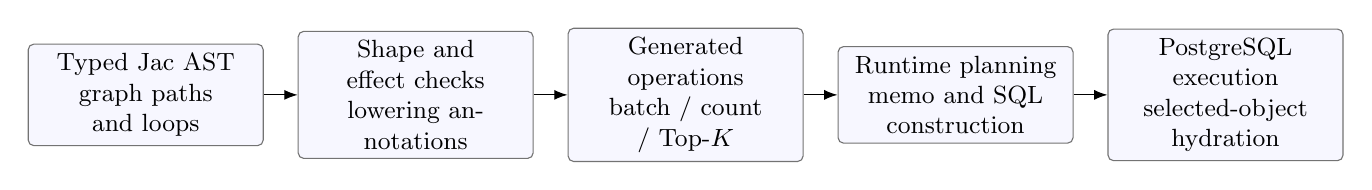
\begin{tikzpicture}[>=Latex,
  box/.style={draw=black!55,rounded corners=2pt,fill=blue!3,
              text width=2.75cm,minimum height=1.0cm,align=center,font=\small},
  node distance=0.43cm]
\node[box] (ast) {Typed Jac AST\\graph paths and loops};
\node[box,right=of ast] (effects) {Shape and effect checks\\lowering annotations};
\node[box,right=of effects] (lower) {Generated operations\\batch / count / Top-$K$};
\node[box,right=of lower] (runtime) {Runtime planning\\memo and SQL construction};
\node[box,right=of runtime] (db) {PostgreSQL execution\\selected-object hydration};
\draw[->] (ast)--(effects);
\draw[->] (effects)--(lower);
\draw[->] (lower)--(runtime);
\draw[->] (runtime)--(db);
\end{tikzpicture}
\caption{Implemented path from graph syntax to relational work. The
application constructs qualifying forum--friend pairs; the runtime submits
their identifiers to the count/Top-$K$ operation. Batch fills complete before
their consuming loops.}
\Description{Five-stage compiler pipeline: typed Jac AST, eligibility checks, generated batch and aggregate operations, runtime SQL planning, PostgreSQL execution and hydration.}
\label{fig:pipeline}
\end{figure*}

\subsection{Batch frontiers before consuming loops}
The compiler recognizes a loop whose body follows an eligible graph hop. It
evaluates the source collection once, materializes the frontier, and emits an
adjacency-prefetch operation for the whole frontier. In the evaluated query,
the predicate \code{joinDate > self.min\_date} accompanies the membership hop.
The walker then consumes individual results from a request-local memo.

Memo keys include the origin, direction, edge and node types, and supported
predicate values. Publishing a memo requires a complete result for the
requested origins. Dirty, deleted, or transaction-modified state restricts
reuse. Where a fast typed fill is eligible, denormalized endpoint types avoid
unnecessary node joins. Ordinary traversal remains the execution path for
shapes outside the recognized or available fast path.

This fill is synchronous: it returns before the consuming loop begins. Its
benefit comes from grouping database work and reusing results. Asynchronous
overlap is a separate scheduling mechanism discussed in
Section~\ref{sec:related}.

\subsection{Recognize a count-and-membership region}
The effect pass identifies a restricted counting family. The outer loop
iterates a two-variable target over \code{dict.items()}; its first statement
initializes a counter. The next loop follows an outbound hop, assigns a second
outbound hop to a local, and conditionally increments the counter based on
membership in a dictionary-indexed set.

The implementation checks that the inner element and its derived local do
not escape, that the counter is observed inside the loop only by the
increment, and that the relevant dictionaries are not otherwise referenced
in disallowed positions. Code generation uses the resulting annotation to
replace the inner counting nest with a runtime count operation. An additional
recognized sort/slice tail selects a count-and-Top-$K$ operation.

These checks capture a useful family of programs whose fields, graph hops,
and accumulator have a direct relational interpretation. They also define a
concrete implementation boundary: eligibility follows the recognized program
shape and the runtime's semantic contract.

\subsection{Relationalize the qualifying pairs}
Let $M\subseteq F\times U$ contain the qualifying forum--friend pairs already
constructed by the application. Let $C$ contain forum-to-post edge occurrences
and $A$ contain post-to-creator relationships. For a candidate forum $f$, the
counting stage computes
\begin{equation}
 c(f)=\sum_{(f,p)\in C}
 \mathbf{1}\!\left[\exists u:\ (p,u)\in A\land(f,u)\in M\right].
 \label{eq:count}
\end{equation}
The sum retains the multiplicity of the traversed container edges. Under the
workload's single-creator invariant, the creator predicate matches the source
test of the first creator.

The runtime deduplicates each membership set and flattens $M$ into UUID
arrays. The database plan first obtains posts authored by the distinct
qualifying members, then matches forum containment and the submitted pairs.
The author-driven intermediate and its containment relation are materialized
in the implemented SQL. This access order can avoid expanding all posts in
every candidate forum. Typed creator scans select Post origins before joining
and exclude Comment-originating edges that share the creator edge type.

The final grouping is joined to the complete candidate-forum key set, so
forums with zero matching posts retain a zero count. The application-supplied
pair relation is both a parameter interface and an explicit boundary between
remaining application work and the relational region.

\subsection{Rank identifiers, then hydrate results}
The Top-$K$ operation combines counts with the required forum ordering in
SQL. Numeric properties use a guarded numeric sort key; textual ordering uses
C collation where applicable. The evaluated tail orders by descending count
and ascending numeric forum identifier.

The compiler also recognizes when candidate forum objects are staged by
identity until that tail. It emits ID-oriented traversal and an ID-only batch
fill, then loads the winning forums with the projected \code{forum\_id} and
\code{title} fields. Ordinary consumers still perform their required
existence, materialization, and access checks. A broader candidate set can be
returned when an ordering projection is unavailable, allowing the retained
application sort and slice to finish the result.

The tradeoff is important: delaying hydration reduces data/object work while
later consumers can introduce additional existence-check statements. The best
execution plan is therefore determined by total work and latency as well as
statement count.

\subsection{Semantic domain}
\label{sec:semantics}
The evaluated counting lowering uses exact edge types, deduplicated membership
sets, zero-preserving candidate keys, and the social-network invariant of at
most one creator edge per post. The syntactic recognizer checks the local
program shape; that schema invariant is supplied by the workload. The count
argument in Equation~\ref{eq:count} depends on it.

The aggregation runtime uses a closure-style permission contract: an
intermediate count can include objects that the requester cannot read
individually, while returned forum objects undergo their normal hydration and
access path. The measured outputs exercise the benchmark's permission domain.
More general permission-sensitive transformations require an authorization
contract that relates intermediate visibility to aggregate observability.

Request-local state, read barriers, and ordinary object consumers remain part
of the execution model. These contracts matter when selecting a relational
region: aliasing, mutation, ordering, cardinality, and permission behavior
determine which observations the transformation must preserve.

\section{Experimental Method}
\label{sec:method}

\subsection{Versions and deployment}
Measurements were collected on October 19, 2026 on an Intel Core i9-10900K
host with 10 physical cores, 20 logical CPUs, and approximately 78\,GiB RAM.
The observed CPU governor was \code{powersave}. The IC5 source A/B compares
baseline \code{c12ba889d} with optimized \code{32c5d1dbb}. Both use the same
unchanged application hash, pinned CPython 3.14.6 build, Jac driver stack,
native PostgreSQL 18.6 instance, and warmed physical structures.

The broader SNB and transaction Jac runs use the optimized revision. The
primary littleX reproduction uses historical revision \code{ad469c988} and
its recovered CONTROL configuration. A separate final-runtime littleX group
retains its own fresh-cell recipe. The write follow-up uses the historical
configuration for three repeated cohorts and additionally measures one
optimized-default cohort on the same historical fixture.

Hand SQL and SQLAlchemy use a dedicated PostgreSQL 16.9 container restricted
to two CPUs and 2\,GiB. The Neo4j 5.26.26 container uses two CPUs and 3\,GiB;
it is stopped before subsequent workload groups. Jac's native database has
the host's resource environment. littleX SQL HTTP servers use CPUs 6--13;
Jac servers and drivers retain the original unpinned placement. Shared
SNB/transaction baselines use the original dependency lock on Python 3.14;
littleX SQL and drivers use their separate original locks on Python 3.13.
Cross-system timings consequently describe these recorded deployments. The
within-Jac source A/B holds the execution stack and backend fixed.

\subsection{Workloads and correctness evidence}
\textbf{Social network.} We use the SF1 data snapshot and parameters associated
with the LDBC Social Network Benchmark~\citep{ldbc}. The implemented IC5-derived
request uses a one-hop friend frontier. We retain that workload definition and
its independently checked SQL reference. The source A/B SQL census executes
20 distinct parameter rows. Logging-off latency uses 40 baseline and 60
optimized IC5 requests. All checked outputs agree with their SQL reference and
historical hashes.

The canonical broader schedule executes 140 warm requests and 2,550 timed
requests per arm: 750 each for IS1--IS3 and 75 each for IC1, IC2, IC5-derived,
and IC13. Each arm's warm-pass 140 result hashes match the reference; all timed
requests complete without errors. This separates response-hash coverage from
the larger timing schedule.

\textbf{Transactions.} A deterministic one-warehouse workload uses New-Order
and Payment operations derived from TPC-C~\citep{tpcc}. Each arm executes
100 mutating warm requests followed by 800 timed requests with plan seed
4242. The complete plan yields 487 successful New-Order operations, 406
Payments, and seven expected rollbacks. Seven database-state checks verify the
final counts, identifiers, warehouse totals, and consistency. Timed New-Order
latencies include six expected rollbacks, giving 443 New-Order-class and
357 Payment samples.

\textbf{Social application.} littleX has 100 users, 50 follows per user, and
20, 50, 100, or 200 tweets per user. W1 returns a full feed; W2 performs
Like, Follow, and Create; W3 mixes a 20-item page with writes at fractions
0\%, 5\%, 15\%, and 30\%. The primary historical-recipe matrix has 40 cells
and 24,000 timed requests. It preserves one persistent SQL server and 12 Jac
cohort servers. Within a W2 tier, Like, Follow, and Create share a seeded
database and process in that order. Each operation has 110 warm and 500 timed
requests; each W3 cell has 110 warm and 1,000 timed requests. Seed-derived
full-feed and page oracles cover all 100 users before restoring the formal
measurement state. Mutation deltas are checked independently. The separate
final-runtime fresh-cell group also completes 40 cells and 24,000 requests.

\subsection{Timing and profiling boundaries}
Generated paper tables use conventional sample medians. The repeated-write
summary is the median of three per-cohort medians; plots show their range.
Original driver statistics and raw samples remain in the artifact. Client
latency measures the complete HTTP operation. littleX's Jac server headline
excludes response serialization, whereas the SQL handler starts its timer
after JWT authentication. Tables identify the metric being compared.

SQL census, logging-off latency, protocol logging, and function profiling run
in separate windows. Before the IC5 census we provision and warm the relevant
physical structures and require zero structural SQL in the measured window.
Projection memos are process-local and must warm again after a server restart.

For writes we collect application/backend CPU, stage headers, complete
multiline SQL, protocol Parse/Bind/Execute durations, and selected function
wall/thread-CPU spans. Separate main-thread and worker-thread cProfile outputs
retain call graphs and counters. Matched controls quantify instrumentation
overhead. DML is also replayed with \code{EXPLAIN (ANALYZE, BUFFERS, WAL)} in
rollback-only disposable databases cloned from the matching seeds.

\section{Results}
\label{sec:results}

\subsection{The IC5-derived source A/B}
\begin{table}[t]
\caption{IC5-derived source A/B. SQL totals use a separate 20-input warmed
census. Latencies are logging-off client medians; the final column is the
paired hand-SQL median during the respective timing window.}
\label{tab:ic5}
\centering\small
\setlength{\tabcolsep}{4pt}
\begin{tabular}{lrrrr}
\toprule
 & SQL total & Latency $N$ & Jac ms & SQL ms \\
\midrule
\tableinput{generated/ic5.tex}
\bottomrule
\end{tabular}
\end{table}

\begin{figure*}[t]
\centering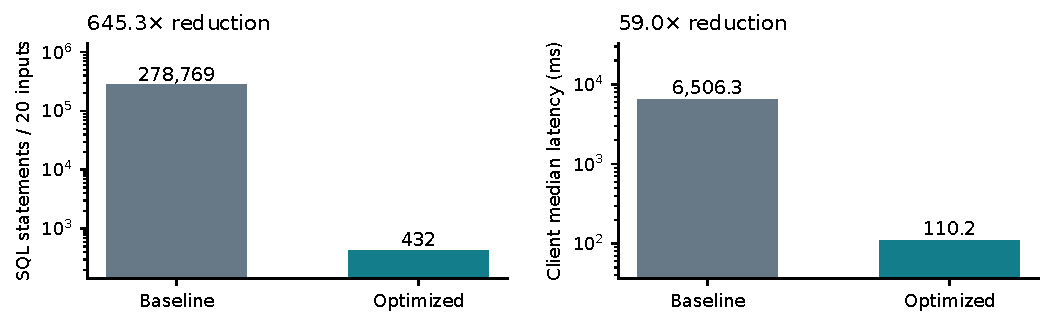
\includegraphics[width=.94\textwidth]{figures/ic5.pdf}
\caption{Source A/B: \SQLReduction{}$\times$ fewer SQL statements and
\LatencySpeedup{}$\times$ lower median client latency. The two panels use
different schedules, as specified in Table~\ref{tab:ic5}; both vertical axes
are logarithmic.}
\Description{Two logarithmic bar charts showing 278769 versus 432 SQL statements and baseline versus optimized client latency of 6506.320 versus 110.206 milliseconds.}
\label{fig:ic5}
\end{figure*}

Table~\ref{tab:ic5} and Figure~\ref{fig:ic5} show the central result. The
baseline executes 278,769 statements over 20 inputs. The optimized runtime
executes 432, with all 20 outputs matching and zero structural SQL in either
census window. The reduced statement volume is accompanied by a decrease
from \BaseLatency{} to \FinalLatency{}\,ms in logging-off median request
latency.

The application is unchanged across this comparison. Source inspection
identifies the changed work: the baseline misses the relevant nested
prefetch/counting shape, while the optimized path batches the qualifying
frontier and replaces per-post creator resolution with an aggregation.
Selective materialization avoids loading all candidate forum objects.

The aggregate statement totals match the historical source A/B. Individual
request counts can also include periodic schema checks and identity lookups.
An additional timed probe records 29, 27, and 29 statements for repeated calls
to one parameter row; removing the observed guard and identity lookup yields
27 each time. The raw census therefore measures complete database commands,
including request maintenance, rather than just the lowered graph operation.

The paired SQL median changes from 45.425 to 57.266\,ms between the source A/B
latency windows. The optimized Jac median remains above its paired SQL
reference. These measurements support the large within-Jac improvement while
preserving the observed residual gap and the variation between measurement
windows.

\subsection{Seven query classes}
\begin{table}[t]
\caption{Canonical SNB-derived schedule, client median ms.
Jac uses the optimized revision. SQL and ORM share the recorded PostgreSQL
deployment; backend/resource differences are in Section~\ref{sec:method}.
$\dagger$~One-hop IC5-derived workload.}
\label{tab:snb}
\centering\small
\setlength{\tabcolsep}{5pt}
\begin{tabular}{lrrrr}
\toprule
Query & Jac & SQL & ORM & Neo4j \\
\midrule
\tableinput{generated/snb.tex}
\bottomrule
\end{tabular}
\end{table}

All four arms complete the canonical schedule and produce 560 matching
warm-pass hashes. Latency varies across queries (Table~\ref{tab:snb}).
Jac is faster than the recorded SQL arm on IS2, IC1, and IC2. Its simple
IS1/IS3 and IC13 requests retain higher request/runtime costs. The
IC5-derived result is 109.032\,ms in this schedule, compared with
54.462\,ms for SQL and 17.250\,ms for Neo4j. This confirms that a successful
graph-to-relational rewrite can coexist with remaining work in pair
construction, runtime execution, and the generated database plan.

\subsection{Bounded and unbounded social feeds}
\begin{figure*}[t]
\centering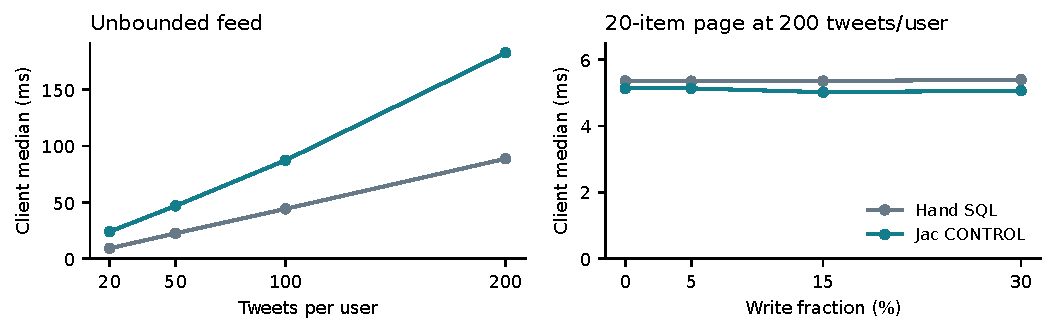
\includegraphics[width=.94\textwidth]{figures/littlex.pdf}
\caption{Primary historical-configuration littleX measurements using complete
client latency. Left: full-feed cost grows with tweets per user at fixed
follow count. Right: a bounded 20-item page at the largest tier remains near
5\,ms as the write fraction changes.}
\Description{Full-feed client latency increases with tweets per user; bounded-page client latency stays near five milliseconds across write fractions.}
\label{fig:littlex}
\end{figure*}

The full feed contains 1,000 to 10,000 tweets per user as the tier increases.
Its cost grows substantially, with Jac retaining a larger client latency than
SQL (Figure~\ref{fig:littlex}). Bounded pages behave differently.
Table~\ref{tab:page} shows both the original headline server statistic and
the complete client measurement. Jac's server median is approximately
24--26\% lower; its client median is approximately 4--6\% lower. The
smaller client advantage reflects request work outside the headline timer and
the different timer starts.

\begin{table}[t]
\caption{W3 page requests at 200 tweets per user, primary historical
configuration. Each row is the page subset of its original mixed schedule.}
\label{tab:page}
\centering\small
\setlength{\tabcolsep}{4pt}
\begin{tabular}{rrrrr}
\toprule
Writes & \multicolumn{2}{c}{Server ms} & \multicolumn{2}{c}{Client ms} \\
(\%) & Jac & SQL & Jac & SQL \\
\midrule
\tableinput{generated/page.tex}
\bottomrule
\end{tabular}
\end{table}

Two controlled diagnoses clarify initialization effects. First, a separate
final-runtime fixture produces a 23.527\,ms full-feed server median, while
the same runtime on the historical fixture produces 15.296\,ms. Runtime and
lazy-transaction controls on the common fixture stay near 15\,ms. The slow
fixture has missing \code{anchors} planner statistics. Executing only
\code{ANALYZE anchors} on a restored disposable copy reduces its median to
15.312\,ms. Captured plans retain the same SQL, parameters, and indexes but
remove repeated kind-index scanning, reducing one representative execution
from 13.393 to 5.465\,ms.

Second, an early ten-warmup page profile begins inside a two-second retry
cooldown after endpoint-projection initialization times out. Its requests use
a generic join, with a dominant query near 27\,ms. After the original
110-request warmup, the projection is ready and SQL uses the global Top-$K$
path. Continuous page controls then produce 3.630\,ms on the historical
configuration and 3.780\,ms on the final runtime. Physical readiness and
retry state are therefore necessary parts of a reproducible compiler/runtime
measurement.

\subsection{Transaction behavior}
\begin{table}[t]
\caption{One-warehouse transaction workload, client medians over the
800-request timed plan. New-Order includes expected rollback requests.}
\label{tab:tpcc}
\centering\small
\begin{tabular}{lrr}
\toprule
Arm & New-Order ms & Payment ms \\
\midrule
\tableinput{generated/tpcc.tex}
\bottomrule
\end{tabular}
\end{table}

All three arms reproduce the deterministic plan and pass the seven state
checks. They finish with 30,487 orders, 305,500 order-line rows, 9,487 new
orders, 30,406 history entries, summed next-order identifiers of 30,497, and
warehouse YTD of 1,362,049.86, with zero recorded consistency violations.

Table~\ref{tab:tpcc} places Jac between hand SQL and SQLAlchemy for New-Order.
For Payment, Jac is slower than both, including a 27.5\% gap to the ORM. The
broader transaction result is consistent with a system whose read
transformations can reduce large computations while short writes still pay
substantial runtime costs.

\section{Explaining the Write Gap}
\label{sec:writes}

\subsection{Stable repeated measurements}
\begin{figure*}[t]
\centering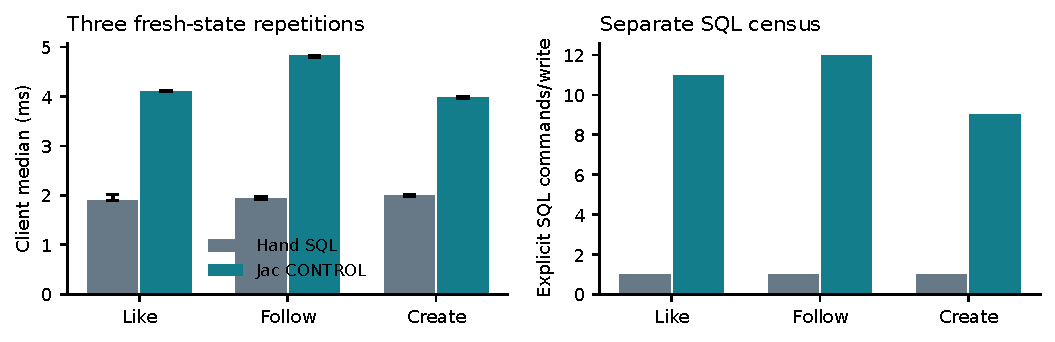
\includegraphics[width=.94\textwidth]{figures/writes.pdf}
\caption{t20 writes. Left: median of three per-cohort client medians;
whiskers show their range (110 warm + 500 timed requests per operation).
Right: explicit SQL commands in separate 100-request protocol captures.
The SQL service's autocommit completion has no separate COMMIT command.}
\Description{Repeated write client medians are about two milliseconds for SQL and four to five milliseconds for Jac, alongside one versus nine to twelve explicit SQL commands.}
\label{fig:writes}
\end{figure*}

We rerun t20 writes in three interleaved fresh-state rounds: SQL--Jac,
Jac--SQL, and SQL--Jac. Each arm preserves the original operation order
and shares its process/state across Like, Follow, and Create. All 18 cells
and 9,000 timed requests pass the count oracles. Figure~\ref{fig:writes} and
Table~\ref{tab:writes} show a stable client-latency disadvantage for Jac.

\begin{table}[t]
\caption{Median of three per-cohort client medians. SQL counts are diagnostic
means; the SQL baseline executes one DML statement per operation.}
\label{tab:writes}
\centering\small
\begin{tabular}{lrrr}
\toprule
Operation & SQL ms & Jac ms & Jac commands \\
\midrule
\tableinput{generated/writes.tex}
\bottomrule
\end{tabular}
\end{table}

A final-runtime cohort on the same historical fixture also passes and
produces client medians of 3.986\,ms for Like, 4.680\,ms for Follow, and
3.807\,ms for Create under the original driver statistic. Thus the complete
request gap persists on the final runtime as well as the historical one.

\subsection{SQL multiplicity and traversal work}
Every profiled historical Jac request executes a main-thread BEGIN, SET,
and two anchor loads. Its worker performs further loads, traversals, anchor
upsert, type-registry insertion, and COMMIT. Complete multiline reconstruction
finds 9 commands per Create, 12 per Follow, and 10.96 per Like. The SQL arm
performs an UPDATE for Like and an INSERT for Follow/Create.

\begin{table}[t]
\caption{Lightweight spans: calls/request / mean driver wall ms per request,
100 requests per operation. Main-thread SQL is additional. Categories partition
\code{PgStore.\_run} calls; surrounding inclusive function times overlap them.}
\label{tab:spans}
\centering\small
\setlength{\tabcolsep}{4pt}
\begin{tabular}{lrrr}
\toprule
Worker category & Create & Follow & Like \\
\midrule
\tableinput{generated/spans.tex}
\bottomrule
\end{tabular}
\end{table}

Table~\ref{tab:spans} localizes Follow's extra work. It executes two traversals
instead of one and three worker anchor loads instead of Create's one. Its
traversal driver wall is 1.004\,ms, exceeding Create's by 0.553\,ms; traversal
thread CPU increases by 0.068\,ms. Captured full-load batches request individual
UUIDs. The measurements establish additional traversal and single-object
loads, rather than assuming that the entire neighbor set is hydrated.

Driver wall includes conversion, query handling, and waiting. Protocol
durations and thread CPU expose different parts of that boundary. Command
counts quantify database interactions; they are distinct from packet counts
or a measurement of network latency.

\subsection{Initialization and object processing}
A lightweight full-dispatch capture measures approximately 1.02--1.07\,ms
main-thread CPU per request and 0.82--1.10\,ms worker CPU. Main-thread
\code{Session.batch\_get} accounts for approximately 0.49--0.51\,ms wall and
0.36--0.37\,ms CPU. Profiling only the walker omits a substantial part of the
application execution.

The call graph also identifies two synchronous TOML parses per request.
Session initialization obtains promotion settings and lease construction
obtains retention settings through separate calls to \code{\_toml\_section}.
Lightweight spans measure 0.154--0.181\,ms wall and 0.155--0.182\,ms thread
CPU for those calls together. This fixed overhead is a concrete caching
opportunity for an appropriately versioned configuration policy.

The heavier profiler records 208--209 archetype attribute assignments per
request, including generated constructors, Session/Store/context setup, and
response handling. These counters identify object-management work across the
request. Its CPU totals include the cost of instrumenting those frequent
calls, so the lighter spans determine the reported timing boundary.

\subsection{Mutation execution and commit}
\begin{table}[t]
\caption{Median summed DML execution over three EXPLAIN replays per
operation on disposable seed clones. Each replay rolls back; COMMIT is
outside this measurement.}
\label{tab:dml}
\centering\small
\setlength{\tabcolsep}{4pt}
\begin{tabular}{lrrr}
\toprule
Operation & SQL DML ms & Jac DML ms & WAL B (SQL/Jac) \\
\midrule
\tableinput{generated/dml.tex}
\bottomrule
\end{tabular}
\end{table}

The captured Jac DML executes in about 0.1\,ms
(Table~\ref{tab:dml}). Its plans record zero trigger executions and zero
shared-buffer reads. The statements generate more WAL than their relational
counterparts, but their short execution times direct attention to the
additional access and request work. WAL volume alone does not identify the
cause of a millisecond-scale request gap.

The worker's explicit COMMIT call takes approximately 1.4\,ms wall and
0.03--0.05\,ms thread CPU in lightweight spans. The SQL service uses
autocommit; transaction completion is included in its database call and is
not a separate COMMIT log event. A separate logged one-row INSERT+COMMIT probe
measures medians of 1.240\,ms for the SQL PostgreSQL instance and 1.211\,ms for
the native instance, with \code{fsync} and \code{synchronous\_commit} enabled.

\subsection{Instrumentation and historical comparison}
Matched 100-warm/100-timed controls compare the same operation plan and cohort
boundaries. Stage/CPU instrumentation increases Jac client medians by
approximately 9--14\%, SQL duration profiling by 18--24\%, and full function
profiling by 145--166\% relative to the uninstrumented control. The detailed
profiles explain executed work; the uninstrumented repetitions establish
the request latency.

The historical t20 report places Jac slightly ahead of SQL. Its SQL and Jac
completion timestamps for the same operation are approximately 44 minutes
apart, and its SQL t20 writes are already flagged as 34--36\% slower than the
earlier banked SQL measurements. Available historical summaries establish
that variation. The current repeated experiment establishes the present
ordering and its execution costs. Identifying a specific cause for the old
ordering requires the corresponding historical per-request and host traces.

\section{Research Implications and Next Steps}
\label{sec:discussion}

\subsection{Optimization units should include dependencies}
The read results show the value of a region that contains a traversal, a
predicate, aggregation, ordering, and materialization policy. The write
results identify a similar opportunity around mutations: resolving a
profile/target, testing a relationship, changing a field or edge, and
persisting the result currently remain several operations.

A next compiler design can represent these operations in a dependency graph
with data, control, effect, and location edges. Each database-derived value
would carry its origin, type, relevant ordering/multiplicity, and permission
requirements. A relational region could begin when its external inputs are
available and its effect/transaction prerequisites have been satisfied. This
design would make cross-ability opportunities explicit while preserving the
observations associated with each walker arrival.

The present implementation supplies concrete lowering targets and measured
costs for such a design: typed hop, membership test, count, Top-$K$, field
projection, hydration, and graph mutation. Its current specialized
recognizers can serve as examples for a more systematic region analysis.

\subsection{A programming-model contract is an optimization input}
Typed relationships and explicit traversal continuations expose information
that an optimizer can use. Turning that information into performance requires
an eligible transformation, a precise semantic contract, suitable physical
structures, and an economical runtime boundary. The unchanged-source A/B
isolates this distinction: the programmer's graph representation is fixed,
while compiler/runtime decisions change the work performed.

The remaining write overhead suggests prioritizing coalesced graph access
around mutations, reuse of request-invariant metadata under explicit
invalidation, and configuration caching. The measured traversal and load
costs provide a basis for choosing those priorities. Schema cardinality and
authorization summaries would also let the compiler determine a broader
semantic domain for aggregate and cross-ability transformations.

\subsection{Evaluation scope}
The reported experiments characterize warm, single-client latency on SF1,
one warehouse, and a small social-application population. The selected
20-row parameter subset, workload-specific schema constraints, container
limits, backend versions, and HTTP stacks define the observed workload and
deployment. Concurrent clients, cold start, larger data, and additional
private-data/cardinality patterns are natural next evaluation dimensions.

The measurements already establish three distinct facts: the source A/B
substantially reduces database work; the broader deployment comparisons are
query-dependent; and the current short-write path has stable, measurable
runtime overhead. Additional ablations can isolate the incremental benefit of
each read rewrite and test the gains from individual write-path changes.

\section{Related Work}
\label{sec:related}

\textbf{Application-to-query compilation.}
QBS derives relational specifications from imperative application fragments
using synthesized invariants and postconditions, then emits SQL
\citep{qbs}. Its ordered-relations treatment emphasizes that moving work
requires preserving the application's result order as well as its contents.
\jacdb{} uses a typed graph interface and concrete compiler recognizers for
frontier and count/ranking computations. Both expose application work to the
database optimizer; their extraction mechanisms and supported semantic
domains determine their respective coverage.

\textbf{Dependent SQL and stored procedures.}
WeBridge uses concolic execution to recover dependent SQL behavior on hot web
application paths and synthesizes stored procedures integrated through the
database-access layer~\citep{webridge}. This addresses the same critical-path
problem created by dependent database operations. The Jac implementation here
uses compile-time graph/loop information and runtime relational operations;
cross-ability dependency analysis is a further direction for that interface.

\textbf{Relationalizing imperative database code.}
Froid transforms imperative UDF computations into relational expressions
embedded in the calling query~\citep{froid}. It demonstrates how a relational
optimizer can optimize a larger imperative computation once the compiler
has supplied a compositional representation. The application-side graph
regions studied here present related questions of region formation, values
crossing the boundary, and effect preservation.

\textbf{Traversal planning and prefetching.}
Temporal Trace Graphs (TTG) combine inspectable access paths with explicit
traversal continuation to construct a bounded request-specific graph and
asynchronously prefetch objects during walker execution~\citep{ttg}.
This supplies a planning interface across traversal steps. The synchronous
batch and relational aggregate paths evaluated here emphasize reducing
intermediate commands and materialization. Continuation-aware planning and
region lowering address complementary scheduling and work-granularity
decisions; combining them requires measuring planning cost, overfetch, and
the residual request path.

\section{Conclusion}
\jacdb{} provides an implemented example of compiling persistent graph
computation into coarser relational work. On the unchanged IC5-derived
program, batching, aggregation, ranking, and selective hydration reduce
SQL volume by \SQLReduction{}$\times$ and median request latency by
\LatencySpeedup{}$\times$. Broader measurements show workload-dependent
performance and identify the remaining expense of short writes. The next
optimization opportunity is the dependency region around graph access and
mutation, supported by explicit ordering, effect, location, and permission
contracts and evaluated through whole-request measurements.

\section*{Artifact Availability}
The local artifact accompanies this draft in the \code{reproduction}
workspace. \code{paper/prepare.py} regenerates the numerical tables and
figures from 59 checksummed inputs; \path{paper/generated/inputs.json}
records those paths and hashes. Core and littleX validators independently
check counts, result hashes, schedules, and state oracles. Raw baseline,
protocol, pstats, call-edge, span, EXPLAIN, and intervention outputs remain
in separate versioned directories. Appendix~\ref{sec:artifact} maps the
main results to these groups.

\appendix
\section{Reproduction Map}
\label{sec:artifact}
Paths are relative to \code{reproduction/}. The application hash for the
source A/B is
\begin{quote}\scriptsize\ttfamily
60aa325001594bf900a8ebcfa24dd1d36\\
fa0f00d0fd3fc9589a781f37f9a32a7.
\end{quote}
The source revisions are baseline \code{c12ba889d}, optimized
\code{32c5d1dbb}, and historical littleX \code{ad469c988}. Raw launch
manifests retain full revisions, application hashes, flags, interpreter and
dependency inventories, and process placement.

\begin{description}[font=\normalfont\bfseries,style=nextline]
\item[IC5 source A/B]
\path{results/baseline-census/}, \path{results/final-census/},
\path{results/baseline-latency/}, and \path{results/final-latency/}.
\item[Canonical SNB and transactions]
\path{results/snb-canonical/jac/}, \path{results/locked/}, and
\path{results/tpcc-jac/}. Independent validation:
\path{results/core-artifact-validation.json}.
\item[Primary littleX matrix]
\path{littlex/original-recipe/20261019T193716Z/}.
Additional final-runtime group: \path{littlex/data/} and
\path{littlex/summary/validation.json}.
\item[Repeated writes]
\path{write-investigation/rerun-baseline.json}; its raw references cover
three rounds and 9,000 timed samples. Separate final-runtime cohort:
\path{littlex/w2-investigation/20261019T212804Z-final-baseline/}.
\item[SQL and function profiles]
\path{write-investigation/sql-work-20261019T212529Z.json},
\path{write-investigation/matched-overhead.json}, and
\path{littlex/WRITE_FUNCTION_SPANS.md}. Corrected category capture:
\path{littlex/w2-investigation/20261019T213148Z-spans/}.
\item[DML and controlled interventions]
\path{write-investigation/dml-summary.json},
\path{littlex/ANALYZE_PLAN_RECEIPT.md}, and
\path{littlex/PAGE_BRANCH_RECEIPT.md}.
\end{description}

\bibliographystyle{ACM-Reference-Format}
\bibliography{references}

\end{document}
